\documentclass[11pt]{article}
\newcommand\tab[1][1cm]{\hspace*{#1}}
\newcommand\back[1][-3cm]{\hspace*{#1}}
\usepackage{graphicx}
\usepackage{soul}
\graphicspath{ {./eprog/} }
\begin{document}
\title{introduction to programming}
\section{objects and classes}
\subsection{object}
Is a software machine that allows other elements to access (query) and modify (command) a collection of data. F.e an object can represent a city or a button.
\\\\Each object belongs to a class that defines the features or operations one can call on this class. It allows other software to access data on modify data on this object (read/write).
\\ An object is an instance of a class.
\\ Objects only exist during the runtime of a program.
\subsubsection{object oriented programming}
In object oriented programming you model objects of the real world into physical/abstract or software object.
\subsection{class}
A class is a sort of category for an object. All objects of a class share the same properties (a class is like a category of things, type).
\\ A program is a model.
\\ A class is the generating class of an object.
\\ Classes only exist in the software text.
\subsection{architecture}
Architecture is the design of a program into it's classes and the relations between them.
\subsection{implementation}
Writing the instructions (algorithms) and data structures of the classes.
\section{interfaces and information hiding}
\subsection{clients and suppliers}
A client of a software mechanism is any sort of system that uses it. f.e person or other software(electronic system).
\\ The software mechanism is the supplier to the system. f.e. class or group of classes.
\\ Arrow always goes from client to suppliers.
\subsection{interface}
An interface is the description of the techniques enabling clients to use it.\\
A program interface is an interface where the client is other software. API: Abstract Program Interface. 
\subsection{API's}
Objects are characterised by the operations clients may apply on them.
\paragraph{queries}
Operations that return the state or information of an object.
\paragraph{commands}
Operations that change the state of an object.
\\\\ The interface is how we (the client) are going to see the object.
Most of the time we do not wan't to see the implementation behind an object and we only wan't to see the interface = Information hiding.
\paragraph{information hiding}
The designer of the class must decide which properties are accessible to the clients and which are internal(only for the purposes of the class itself (public and secret)).
\section{Commands and queries, uniform access principal}
\subsection{Features: commands and queries}
Every feature call, will always be called on a object (your\_object.your\_feature). A feature is an operation available on a certain class of objects. Their are three kinds of features:
	\\Commands\\Queries\\Creation procedures
	\paragraph{Queries} calling a query should not change the answer the program gives back! The goal of a query is to obtain information about the object without modifying it.
	\paragraph{Commands} change the properties of one or multiple objects.
\subsection{Routines, procedures, functions, attributes, and the Uniform Access Principle}
\subsubsection{Routine (=method )}
Removing details specifics and capturing the essence of the information.\\ In programming there are two sorts of abstractions: \\Data abstraction, done with a class.\\Computational abstraction (algorithms) done with routines.\\Example of a routine in Eiffel:\\r(arg: type)\\require\\\tab preconditions...\\do\\\tab instructions...\\ensure\\\tab  postconditions...\\end
\subsubsection{Uses of routines}There are two different uses for Routines:\paragraph{bottom-up:} Encapsulating a computation for reuse.\paragraph{Top-down:} Calling a routine before having written it. Allows to write the bigger code at the beginning and go to the little details later.
\subsubsection{Kinds of routines}
Their are two kinds of routines:\paragraph{Procedure:} doesn't return a result.\paragraph{Function:} returns a result(f(arg: type):result type).\\
\back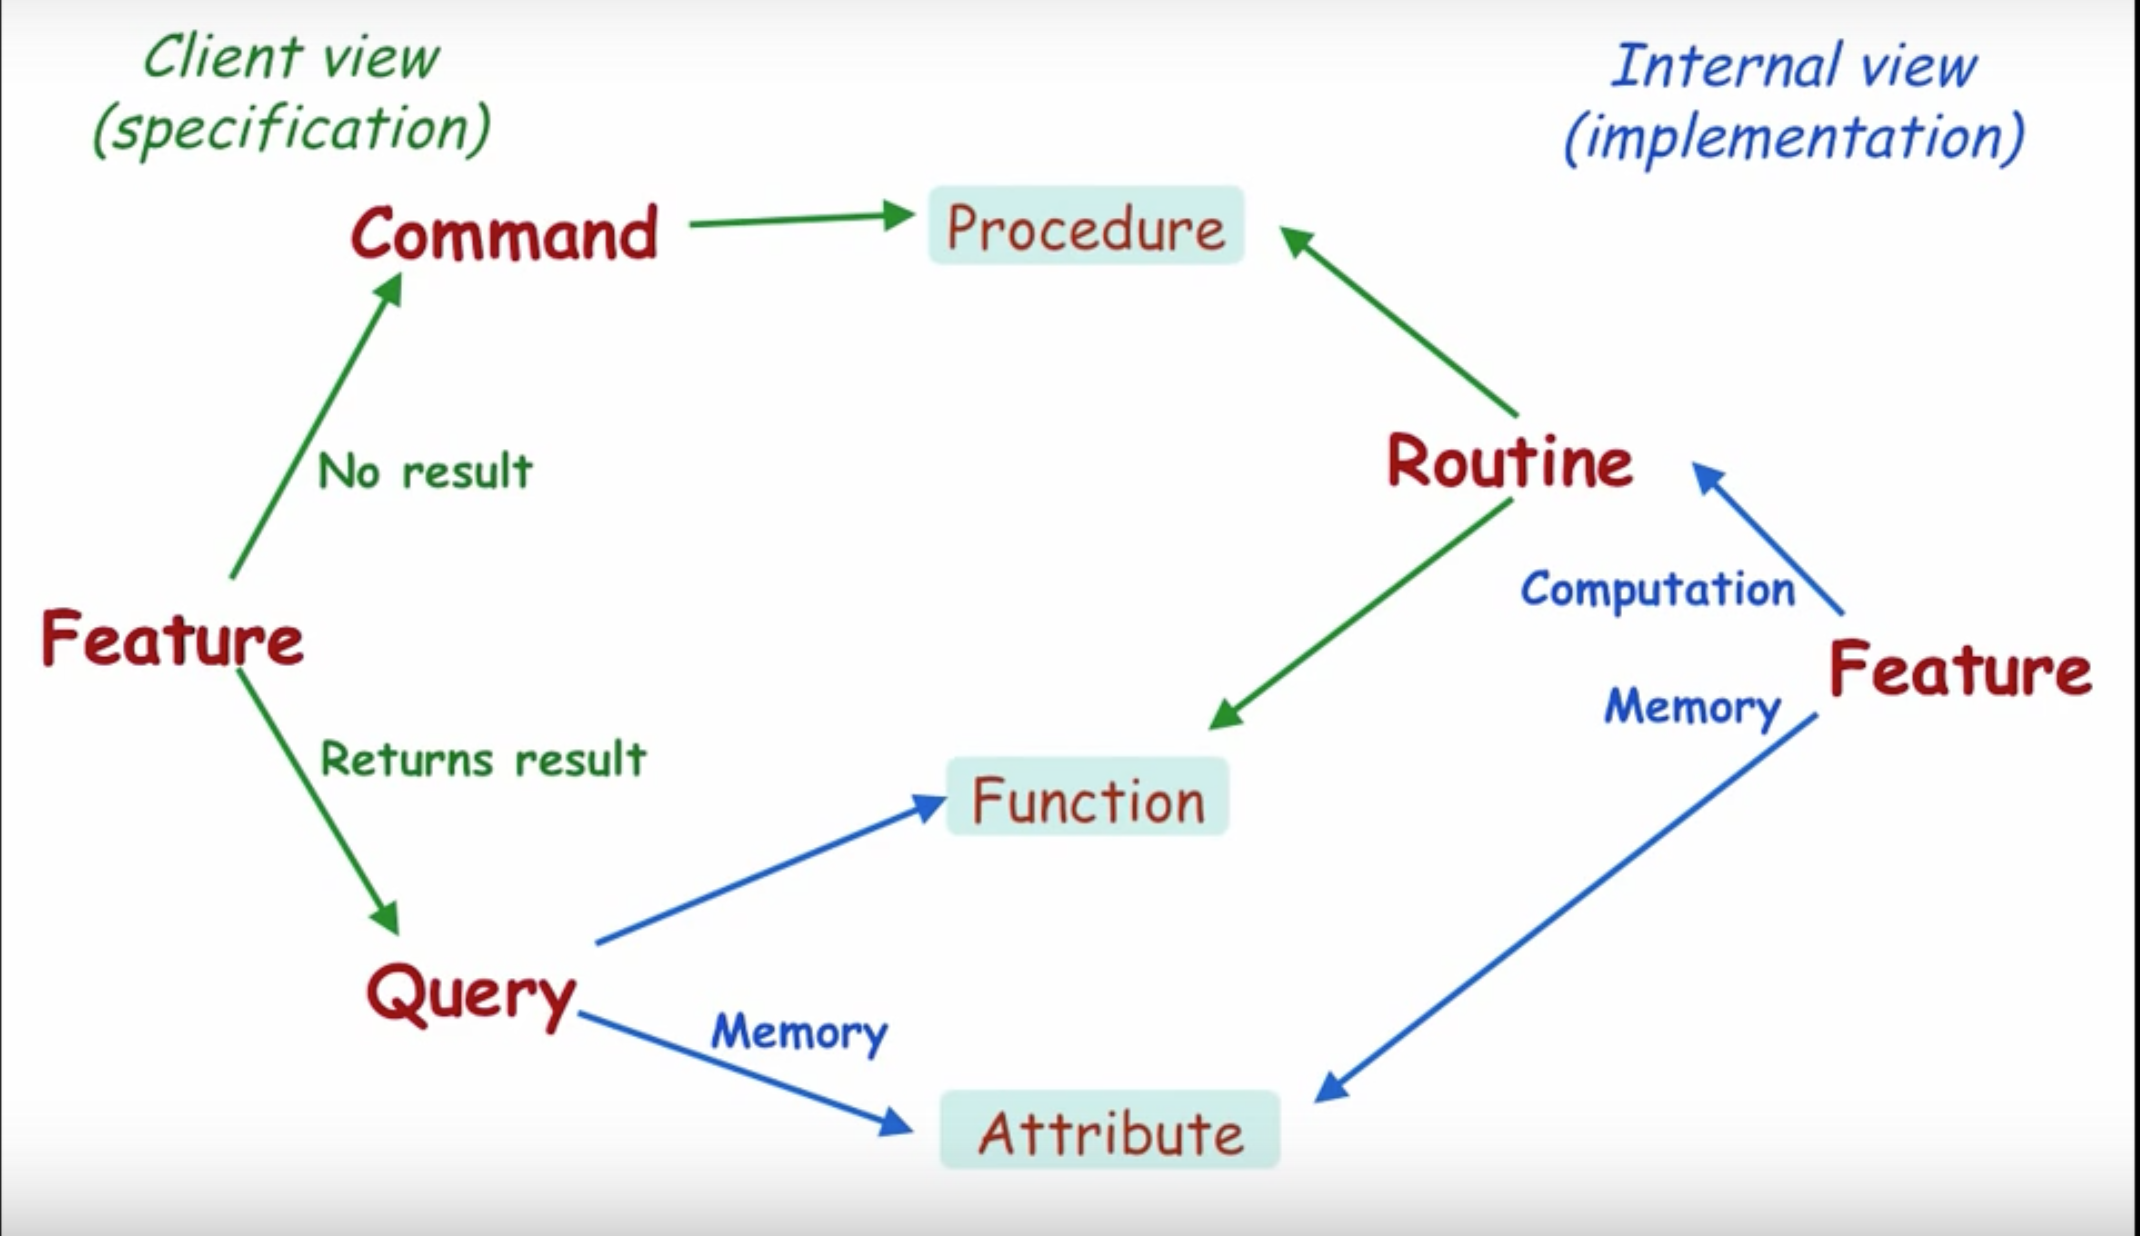
\includegraphics[scale = 0.5]{feature}
\subsubsection{Attributes}
Each class has an attribute field where there is every object of this class in the program.
\subsubsection{The uniform access principal}
Features should be accessible to the client in the same way wether implemented by storage or by computation(it does not matter if what you are looking for already exists in the memory or if you have to compute it from some other pieces of memory(in the image function and attribute are therefore equal)). 
\section{Object creation}
\subsection{basics}
\subsubsection{Identifier}
An identifier is a name chosen to describe certain elements of the program such a class, feature or object.\\ An identifier that denotes a value at runtime is called an \hl{entity}.\\ If the value of an entity can change during runtime it is called a \hl{variable}.\\ An entity detonating an object is \hl{attached} to this object. 
\subsubsection{Object creation}
First you create an object in memory and then attach an entity to it. First you have to declare the entity with a certain type (leg1: LEG). Then you create leg1(create leg1). Leg1 will then be created during runtime and initialised with the default values.\\ If you want to create an object with other than the default values, you can create \hl{creation procedures} for the class.\\\\class point create\\\tab default\_create, make\_cartesian, make\_polar\\feature\\\tab...\\end\\\\ You then have to declare these creation procedures in the feature. Then you can declare the object as(create point.make\_polar(r,t)) (create point == create point.default\_create).
\subsection{Void references}
\subsubsection{Initial state of an object}
Initially, before the creation of an object, it's reference is void. During execution a reference is either \hl{void} or \hl{attached}(to find out you can write x=void or x/=void).
\subsubsection{Utility of void references}
For example in a linked list, to know where the list ends the next next reference of the last element of the list is void.\\ Void references do cause trouble however \hl{(you cannot call a feature on a reference wich is void)}. Eiffel is void safe, therefore the code will not compile if the code might cause a void call.
\subsection{Object creation and the system root}
\subsubsection{How it all starts}
Executing a system is the creation of a \hl{root object}, this is an instance of the \hl{root class}, using a special creation procedure of this class called a \hl{root procedure}. In every program you have to choose a root class and a root procedure(main class in java).
\subsubsection{Current object}
Is the latest object on which an operation was started. There is always a current object during execution, initially it is the root object(this in java). When you call x.f(a), x becomes the new current object, after it has finished executing the current object before it was x becomes the current object again.

\section{References, Assignment, and Object Structure}
\subsection{Objects, values and references}
\subsubsection{Object structure}
An object is made out of fields, each field has a value which is either a \hl{basic value} or a \hl{reference}.
\subsubsection{Types} There are also two kinds of types, \hl{reference} where the entity has a reference to it's type, or \hl{expanded} where the entity is it's type (an expanded type can not be void since it corresponds to an object). Many objects can have a reference to the same type, but expanded type cannot share.\\ In order to get expanded objects, the classes have to be declared as expanded:\\\\ expanded class E\_STATION\\\\All classes such as integer, boolean, character etc.. are all expanded classes.
\subsubsection{Initialisation}
Their are automatic initialisation rules:\\\tab 0 for numbers\\\tab null for characters\\\tab false for booleans\\\tab void for reference\\
\subsubsection{Strings}
Strings are actually and object in eiffel and java. Therefore the field containing a String in an object will be a reference field.
\subsection{Kinds of feature calls and the client relation}
\subsubsection{Attributes}
The fields of a class reflect it's attributes.\\ To set a field: x:=new\_x(= in java (instruction))(= is equal to == in java(expression)). The value of the field is then changed or the reference.
\subsubsection{Feature calls}
There are two types of feature calls: \hl{qualified} and \hl{unqualified}.
\paragraph{Unqualified call} when the feature is being called on the current object (set(new\_x, new\_y) or Current.set(new\_x, new\_y)).
\paragraph{Qualified call} the feature is being called to a different object and this object becomes the new current object (position.set(new\_x, new\_y)).
\subsubsection{The client relation}
If a class has a field that is a reference to another class and features calls on this field with feature from the other class. The first class is a client of the second.
\subsection{Assignment}
\subsubsection{Entities}
An entity is a name in the program that denotes run-time values.\\ Some entities are \hl{constant} and others are \hl{variables}: attributes or local variables.\\ changing a variable value: target:=source\\ The target may be an attribute, a result of a function or a local variable. A source a call to a query or an arithmetic expression.
\subsubsection{Unreachable objects}
When a field in the memory has no reference to it.\\There are two approaches to this problem: Manual(c++,Pascal) the programmer has to take of this, Automatic garbage collection (eiffel, java).
\subsubsection{Assignments}
Two types of assignments: reference(replaces the reference with another one (or void)) and expanded(copies the value).
\subsubsection{Local variables}
Local variables are entities that only exist inside a routine. Declaration:\\\\require\\\tab ...\\local\\\tab x: Real\\do\\\tab ...\\ensure\\\tab ...\\end\\\\ In this case x is a local variable.
\section{Logic}
\subsection{Boolean logic}
\subsubsection{boolean expressions}
In a boolean expression there are: boolean variable (denoting boolean values) and boolean operators (not, or, and, =, implies).\\Truth assignment for a set of variables is a choice of true or false for every variable.
\subsubsection{Tautologies}
A tautology is a boolean expression that has true for every possible truth assignment.
\subsubsection{Contradiction}
A contradiction is the opposite of Tautology.
\subsubsection{Satisfiable}
An expression is satisfiable if for one truth assignment it is true.
\subsubsection{De Morgan's laws}
You can use these laws to simplify boolean expressions.\\ and and or are associative: a and (b and c) = (a and b) and c. The same for or.
\subsubsection{Implies}
Implies is only false if a implies b if a is true and b is false.\\a implies b = not b implies not a.
\subsubsection{semi-strict operators and quantifiers}
\subsubsection{semi-strict boolean operators}
If you divide by x you get an undefined result if x = 0. Therefore you want to check if x = 0 before you do the division and so you need a \hl{non-commutative} version of and and or: \hl{semi-strict boolean operator}.
\\\hl{and then} = semi-strict version of and.\\\hl{or else} = semi-strict version of or.\\semi-strict boolean operators allow you to use an order in boolean expressions.\\
a implies b =  not a or else b (implies is always semi-strict).
\subsubsection{Universal quantifiers}
Universal quantifiers are \hl{there exists} and \hl{for all}.\\On a empty set: there exists is always false and for all is always true.
\section{Control Structures}
\subsection{Basics and compounds}
\subsubsection{Algorithms}
An algorithm is a process to be carried out by a computer.\\ The difference between an algorithm and a program is that an algorithm is more abstract independent of a platform and a programming language. A program normally contains multiple algorithms. Programs are the combination of data structures and algorithms.
\subsubsection{Control structures}
\paragraph{Definition:}
 program construct that describes the scheduling of basic actions.\\\\There are three fundamental control structures: \\\tab sequence\\\tab conditional\\\tab loop\\they are the control structures of structured programming.
\paragraph{Sequence}
to achieve c form a, I first achieve b from a, and then c from b.
\paragraph{Conditional}
Solve the problem separately on two or more subsets of the input set.
\paragraph{Loop}
solve the problem on successive approximations of its input set.
\subsubsection{Correctness of a compound}
Are done with post and pre condition.\\The postcondition an instruction must imply the precondition of the next instruction.
\subsection{Conditionals}
\subsubsection{Structure}
if\\\tab condition\\then (or if condition then)\\\tab instructions\\else (elseif) \\\tab other instructions\\end
\\You can combine conditional instructions in other ones: \hl{nesting} but it is better to just use elseif.
\subsubsection{Multi-branch statement(case)}
\hl{Structure:}\\\\
inspect expr(character or integer)\\\tab when value1 then\\\tab\tab instruction1\\\tab when value2,value3 then\\\tab\tab instruction2\\\tab when value3..value5(anything between value4 and value5) then\\\tab\tab instruction3 \\\tab else\\\tab\tab other\_instruction\\end\\\\
The inspect table stops as soon it reaches one that is true.\\ You have to write the else on the end of multi-branch or it will cause an exception if it goes to the end.
\subsection{Loops}
\subsubsection{Structure}
from\\\tab initialisation\\invariant\\\tab invariant expression\\variant\\\tab variant expression \\until\\\tab exit condition\\loop\\\tab body\\ensure\\end\\\\
The loop will keep on going until the exit condition becomes true. invariant and variant are optional.
\subsubsection{Operations on a list}
When we have a list there is a cursor which gives us the current position in the list.
\paragraph{Commands}on lists\\
\tab start\\\tab back\\\tab forth\\\tab count\\\tab before\\\tab after\\ start = position 1, before = position 0 and after = position count + 1.\\ there for in a loop you can write:\\from \\\tab line.start\\until \\\tab line.after\\loop\\\tab line.forth\\end\\
\subsubsection{Across loops}
An across loop is a more compact way to write a loop that traverses a structure:\\across structure as c loop\\\tab do something with c.item\\end\\
\subsubsection{Other loop types}
these are not available in eiffel\\
while condition(while this is true (inverse to normal loop)) do\\\tab body\\end\\\\
repeat\\\tab body\\until \\\tab condition\\end\\\\
for i:a..b (i form a to b) do\\\tab body\\end 
\subsection{Loop invariants and variants}
\subsubsection{Invariants}
The invariant helps to check that if the loop terminates it fulfils it's goal and is a \hl{boolean expression}. The variant helps to check that the loop will terminate. The loop body will always be very tightly tied to the invariant.\\The invariant can be seen as the set in which the loop operates and the loop can never exit this set. Therefore the body must preserve the invariant.\\The conjunction of the invariant and the exit condition gives us the effect of the loop.
\subsubsection{Variants}
Invariants are used to ensure that loops will terminate and is an \hl{integer expression}.\\The integer expression must be:\\\tab non negative after initialisation\\\tab decrease while remaining non negative for every iteration of the body\\\tab executed with exit condition not satisfied.\\For example in a loop that traverse a list the invariant would be:\\\tab list.count - list.index + 1\\The \hl{Entscheidungsproblem}: the fact that no compiler will be able to tell if a loop will terminate(Alan Turing).
\section{Single inheritance}
\subsection{Single inheritance}
\subsubsection{Classes}
Classes can be viewed in two different ways, as a \hl{module}(groups a set of services), or as a type. As a module it has a set of features and as a type it has a series of runtime instances.
\subsubsection{Inheritance basics}
Describing a new class as a extension or specialisation of an existing class(or several with multiple inheritance).\\If B inherits from A,:\\ as modules :\hl{all features of A are available in B}.\\ As types: \hl{whenever a type A is needed a type B will also be acceptable}.\\In this case B is a \hl{heir} of A and A is a \hl{parent} of B.\\The \hl{descendants} of A are A and the descendants of A's heirs.
\subsubsection{Declaring a heir class}
class\\\tab class name\\inherit\\\tab this class's parent\\feature\\end 
\subsubsection{Features}
An \hl{immediate feature} is a feature declared in a class itself or it can be a \hl{declared feature}.
\subsection{Polymorphism}
Related to the type view of inheritance(polymorphic = multiple types).
\subsubsection{Polymorphic assignement}
If you have a reference object initialised as an object of type T where, A and B inherit from T. You can change the reference of T to either A or B(however you cannot call a feature defined in A or B on T even after you have changed it's type because of the compiler).\\For example if you have a class transport, a class taxi and a class car. If T is of type transport, you can then change T to be of type car or taxi, according to the choice of the client for example.\\\hl{The type of source has to be the descendant of the type of the target} when target := source.
\subsubsection{Static and Dynamic types}
The static type of an entity is the type used in it's declaration.\\The dynamic type of an entity is the type of the object that this entity is attached to, during runtime.\\An entity can only have one static type but can have multiple dynamic types.\\The dynamic type will always conform(is a descendant of) it's static type. A expanded type conforms only to itself.
\subsubsection{Static typing}
When a language is static typed the compiler checks that there will be no type faults. If you call x.f, x will always have a feature f.
\subsection{Dynamic binding}
\subsubsection{Redefinition}
When a class B inherits from a class A, you can redefine a feature that was already declared in the class A to function differently in B.\\class B inherit A\\\tab redefine\\\tab\tab feature\\\tab end\\create\\feature\\invariant\\end\\\\You can not have two features with the same name in A and B.
\subsubsection{Dynamic binding}
With polymorphism we have an object T that may be either it's static type A or it's dynamic type B. Both A and B have a feature T.r where r has been redefined in B. The effect of the call T.r will depend on the dynamic type of T.(Vs dynamic binding which will call the static type feature (c++)).\\Static typing will guarantee that there is \hl{at least one} version of the feature that will be able to be called.\\Dynamic binding guarantees that every call will use the \hl{most appropriate version} of the feature.
\subsubsection{Single choice principle}
If a system supports several variants of a notion, knowledge of the set of variants should be limited to one module(principle behind dynamic binding).
\section{Design by contract}
\subsection{Preconditions}
Expresses what a supplier routine requires to function properly when invoked by the client. The responsibility for a correct invocation lies on the client.\\They are boolean expressions checked every time the routine is invoked.
\subsubsection{Structure}
function()\\\tab require\\\tab\tab precondition\\\tab do\\\tab\tab ...\\\tab ensure\\\tab end\\\\A precondition is generally preceded by a text label to make it more readable, example of a precondition: value\_positive: a > 0 (do not need to write this during the exam waste of time).\\Precondition can be linked together using and, or, not, = implies. Writing two expressions on two consecutive lines is considered as an implicit and. You can also invoke separate boolean expressions that are too complicated or too long to put in the precondition.\\If a client invokes a routine and doesn't satisfy the precondition, an exception will be invoked, the line and the label of the precondition will come in handy.
\subsubsection{Design by contract vs defensive programming}
Design by contract assumes that one should trust clients to invoke a routine correctly. The checks for correct routine invocation are encoded in the supplier using preconditions. The checks can be disabled at runtime if we are sure of the code. Preconditions are intended for scenarios that should never happen(a fail points to an error in the code). Preconditions should be as strong as possible, so that if they do not fail, the program should run as expected.
\subsection{Postconditions}
Expresses what a supplier routine guarantees if invoked properly by the client. Responsibility for a correct result lies on the supplier. Can be disabled if sure that the code is correct.\\They are boolean expressions checked after the execution of the body.\\Postconditions are located after the ensure in the routine. They are the same thing as preconditions otherwise.
\subsubsection{Old keyword}
Old is used to see how a value has changed after the routine body execution. For example: value\_added: value = old value + a\\\\In postconditions we specify what has changed during the execution and how it has changed.
\subsection{Class invariants}
Class invariants express properties that all objects of the class must satisfy.\\They are boolean expressions checked every time a supplier's status is observable by clients, \hl{as soon as an object is created}, \hl{before and after a feature is available to clients}.
\subsubsection{Structure}
class classname\\invariant\\\tab boolean expressions\\\\
they are written the same as preconditions.\\Class invariant are aloud to be broken in these two scenarios: \hl{before the invocation of a creation feature} and \hl{in the body of any routine}. The invariant has to always hold when it matter: \hl{when the values of the object are available to clients via queries}
\subsection{Contracts and inheritance}
This section explains what happens to contracts in inheritance, polymorphism and dynamic binding.
\subsubsection{All you need to know}
We take the point of view of a client C accessing a feature f of class A and redefined in classB that inherits form A.\\The \hl{precondition in the redefined f can only stay the same or be weakened}\\\hl{the postcondition in the redefined f can only stay the same or be strengthened}\\\hl{the class invariant in the descendant class can only stay the same or be strengthened}.\\\\If i want to redefine a precondition of a redefined function f then I have to write:\\f\\\tab require \hl{else} precondition\\\\This new precondition has to be weaker than the old one.\\The similar goes for postcondition but, fi you want to change the postcondition you have to write:\\ ensure \hl{then} postcondition\\\\This postcondition has to be stronger than the old one.\\For invariants, it is similar for the postconditions and you just write new class invariants when writing the class and \hl{the new invariant will be added to those of the parent class}, they also have to be stronger. If you are happy with any of the old post, pre or invariant just dont write require, ensure or invariant.
\subsection{Putting it all together}
For performance, you can enable or disable(also partially) contracts at runtime(disable after program tested).\\Desing by contract allows tests to be generated automatically.\\Contracts should never be used to validate user input(or external sources).\\ Too weak == sound == incomplete, too strong == unsound == complete.
\section{Genericity}
\subsubsection{The problem}
Genericity is a way to reuse code that we have already written.\\It let's us make for example a list of objects without knowing the type of that object and let the list work for any type of Object. Essentially you write the list as if you were writing a list of people for example, but instead of giving the type people you give the type \hl{ANY}. However writing the list in this way we then have a list that contains multiple types of objects, and by inserting an object into this list you loose the information of the object type.
\subsubsection{The solution}
We add a parameter to the class:\\class LIST [G]\\\\feature\\\tab extend(x: G)\\\tab\tab do...end\\\tab item(i: INTEGER): G\\\tab\tab do...end\\\\To declare the list you just have to mention what type the list will be : \hl{cities: LIST[CITY]}
\subsubsection{Constrained genericity}
If we want to put constraints on what type of object can go into our lists for example. If we want to implement a sorted list for example, the object that go into the list have to be comparable. Therefore we will only take objects that inherit form the class COMPARABLE:\\class SORTED\_LIST\\\tab G $\rightarrow$ COMPARABLE (in brackets)
\section{Selective Exports and Deferred Classes}
\subsection{Selective exports}
What can classes do with the attributes of other classes.\\On principal the attributes of a class are read only. In order to allow other classes to change the attributes of another class, \hl{there is no other way than threw a procedure of the first class (getter functions)} (all variables are private but can be seen).\\In Eiffel attributes are seen as queries for outside classes.\\ It is possible to create a getter procedure directly at the creation of an query in eiffel:\\ temperature: REAL assign set\_temperature\\After such declaration the command \hl{x.temperature = 21.5 is allowed as an abbreviation for x.set\_temperature(21.5)};
\subsubsection{Information hiding and selective export}
It is possible to choose what classes will be able to access certain features of a class, to do this:\\class\\\tab A\\feature\\\tab f...\\\tab g...\\feature{NONE}\\\tab h,i...\\feature {A,B,D}\\\tab j,k,l...\\end\\\\ \hl{When you declare feature{NONE} even the class itself where these feature will be declared won't be able to access them. Neither if you don't call this class in the brackets.}
\subsection{Deferred classes}
They allow us the express abstract concepts independently of implementation. \hl{Effective != non-deferred}. \\\hl{Deferred is a class or a feature that is not completely implemented.} 
\subsubsection{Deferred features}
Example of a deferred feature in list:\\forth\\\tab require\\\tab\tab not after\\\tab deferred\\\tab ensure\\\tab\tab index = old index + 1\\\tab end\\Here we don't specify the implementation because it will be different for every kind of linked lists. Most often when you write deferred features you write their pre and postconditions and don't specify there implementation.
\subsubsection{Deferred classes}
A class is deferred if it has at least one deferred feature. The class is declared as \hl{deferred class}, \hl{such a class cannot be instantiated.} A deferred class has a \hl{star} after the name in a schema. High level classes are often deferred.
\section{Recursion}
A data structure is recursive if it is built from smaller pieces of the same data structure.
\subsection{Routines}
A routine has direct recursion if it calls itself and is indirect recursive if it calls another routine which then calls the first routine(the number of levels is not important).
\subsection{Data structure}
A binary tree is recursive because every subtree is also a subtree.
\section{Data structures}
\subsection{containers}
A container is something that can hold other objects. All containers can \hl{insert an item}, \hl{access an item} and \hl{remove an item.} Some containers have key or indexes to find the items more efficiently. Every container data structure is more efficient at some kind of operation.
\subsubsection{Arrays}
Each item has an identifier index.\\
\back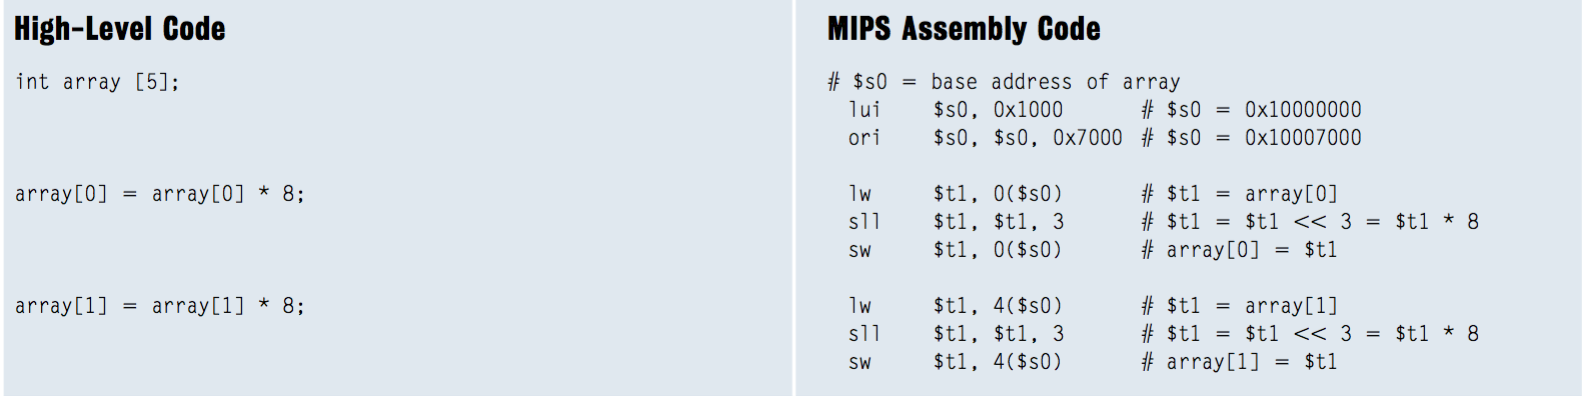
\includegraphics[scale = 1]{array}
\subsubsection{Lists}
A list is a container storing items, identified by an integer index, where items can be inserted or removed at any position. There are two type of lists: \hl{array based} and linked. Array based are similar to array but if you remove a value in the middle then all the elements after it have to be moved 1 space forward, the same if you insert in the middle.\\
\back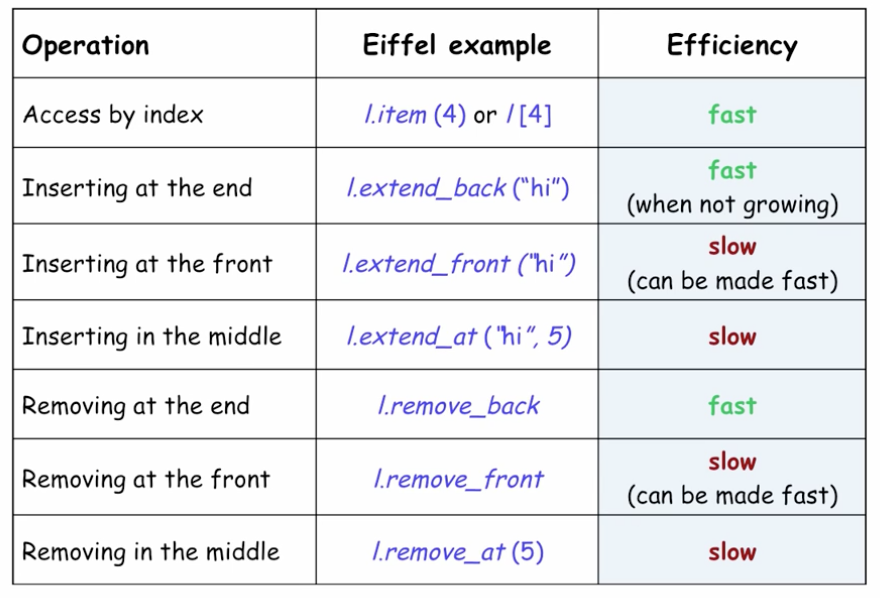
\includegraphics{list}\\
Linked lists have a reference to the next item in the linked list. The reference of the last item is void.\\
\back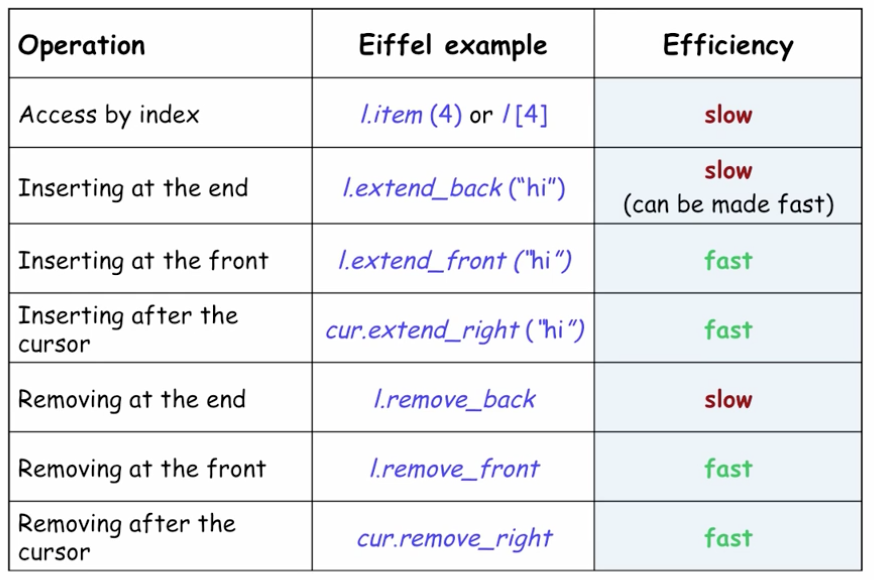
\includegraphics{linked}
\subsection{Stacks}
In a stack you can only access or remove the item on the top of the stack: \hl{LIFO.}\\
\back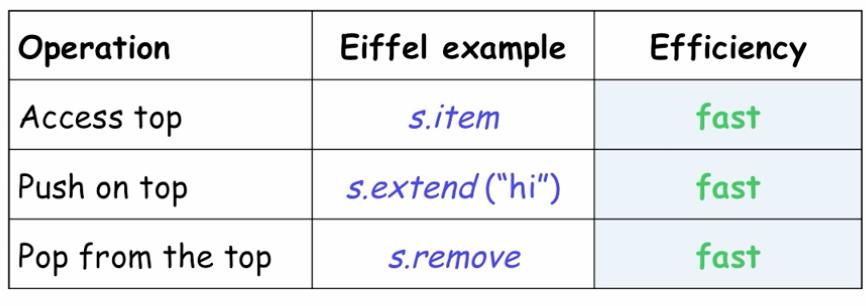
\includegraphics{stack}
\subsubsection{Queues}
Like stacks but you can only access or remove the bottom of the queue: \hl{FIFO\\}. There are also two types of queues: array based(ring buffer) and linked list.\\In the array based you use a ring buffer, and the position of the items loop over the array, the tail and front are somewhere in the array but don't have to be at the top or end. The linked list version is like a normal linked list but you have an extra cursor that points to the tail of the list.\\
\back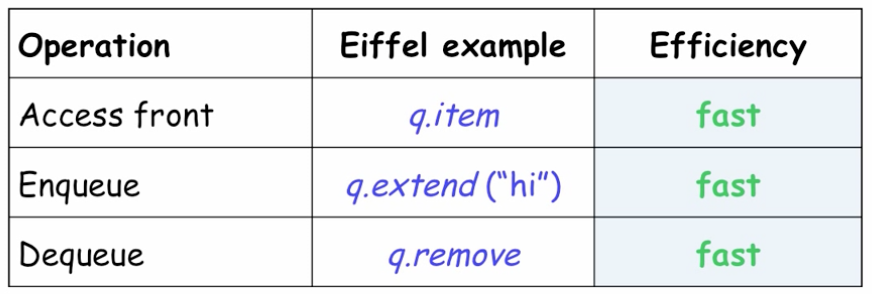
\includegraphics{queue}
\subsection{Tables}
Like arrays but the indexing is not done with integers but with other stuff like strings.
\subsubsection{Hash tables}
Map all possible keys into an integer interval 1..n and then store the items in an array. Problem with this is that it causes collisions. Solutions: open hashing(if there is a collision you create a linked list in this position in the array). Another solution is closed hashing where if a position is already occupied you try another position for example position + 1.\\
\back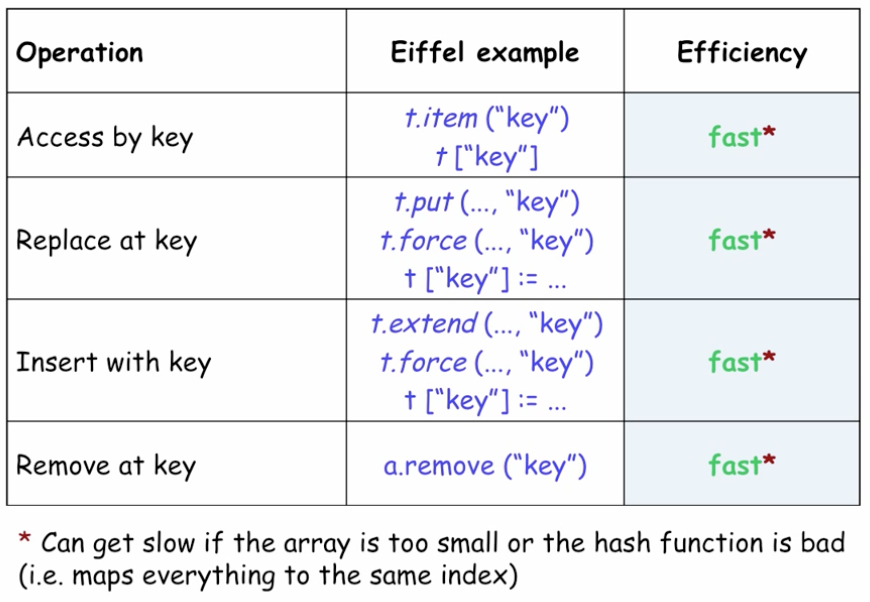
\includegraphics{table}
\section{Multiple inheritance}
\subsection{basics}
A class that inherits from multiple other classes.\\\hl{You can compare the value of two objects with object1 ~ object2, if you write object1 = object2 the answer is if there reference is the same.}\\Example of multiple inheritance:\\class arrayed\_list [G] inherit\\\tab list[G]\\\tab array[G]. There are two ways to get this result. The first one that we have seen, we consider that an arrayed\_list \hl{is} an array and in the second we consider that an array\_list \hl{has} an array:\\class arrayed\_list [G] inherit\\\tab list[G]\\feature\\\tab rep: ARRAY[G]\\the attribute rep represents a field in the list that is an array.
\subsection{Non conforming inheritance}
You can have several inherit clauses in the class and you can have an \hl{inherit {NONE}}. This is non conforming inheritance which makes polymorphism impossible. Is marked in the visualisation of classes with an arrow that has a line threw it.\\ If a class inherits from List and inherit{NONE} from Array, \hl{then you will be able to have a list of array but not an array of lists.}
\subsection{Name clashes}
What happens when a class inherits from two other classes that have features with the same names. The solution is pretty simple you just have to \hl{rename} one of the two features in the new class. This is done with the command: \hl{rename f as A\_f}.\\All name clashes must be removed, \hl{unless} the feature in the two other classes is actually an inherited feature that they both inherit from the same class (repeated inheritance), or at most one of the features is effective and all of the others are \hl{deferred}.\\If the feature is deferred in only one of the two classes then it will be implemented with the expanded feature of the other class.
\subsubsection{Renaming and redefining a class}
class A inherit\\\tab B\\\tab\tab rename f as g redefine g end\\\\You can also use renaming to adapt a name in the new class if the name is ideal anymore, even if there is no name clash.
\subsection{Feature merging and undefinition}
Reminder star = deferred and + = effective and ++ = redefined . 
\subsubsection{Feature merging}
a class D inherits form A, B and C. You want to merge the features that are deferred from A and B with an effective feature form C. To do this you can use \hl{renaming}. You just rename all  the features so that they have the same name and the deferred ones will take the implementation of the effective one:\\class\\\tab D\\inherit\\\tab A\\\tab\tab rename\\\tab\tab\tab g as f\\\tab\tab end\\\tab B\\\tab\tab rename...\\\\
\subsubsection{Undefine}
If you want to forget a feature from a class you can \hl{undefine it.}\\inherit\\\tab S\\\tab\tab undefine v end\\Undefiniton might only work if there is a name clash(seems stupid but is defined this way in the videos), so if you want to undefine a feature you first have to rename it to a name of an existing effective feature of another class and then undefine it.
\subsection{Repeated inheritance}
Repeated inheritance is when a class inherits from two other classes, who themselves inherit from the same class(diamond structure). A class is a descendant from another class threw more than one path.
\subsubsection{Select}
Assume we have B and C that inherit from A and D that inherits from B and C(diamond structure A on the top and D on the bottom). \hl{If the class B redefines features from A and C does not.} Which features do we use in D, the redefined ones or not?\\You have to use the \hl{select clause:}\\inherit\\\tab B\\\tab\tab select\\\tab\tab\tab f\\\tab\tab end\\\tab C\\\tab\tab rename...\\
If the repeated inheritance occurs you have to use the select clause.
\section{16. Functional Programming: Agents}
\subsection{The Model View Controller pattern}
We will extend our control structures(decides what part of the program runs when) with a more flexible mechanism where control is decentralised. Using \hl{agents.}
\subsubsection{Event driven programming}
The user drives the program with different event options he can trigger(mouse keyboard etc...). Vs program driven control.
\subsubsection{Model-view controller}
\back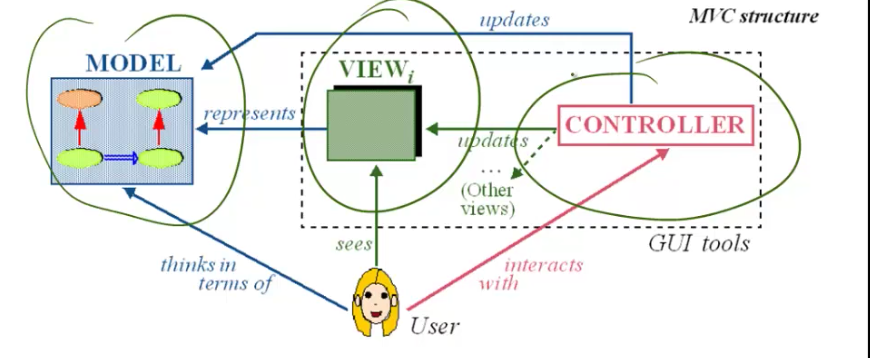
\includegraphics{model}
\subsection{The observer pattern}
A design pattern is an architectural scheme, a certain organisation of classes and features, that provides applications with standardised solution to a common problem.\\
\subsubsection{Publisher subscriber, observer pattern}
\back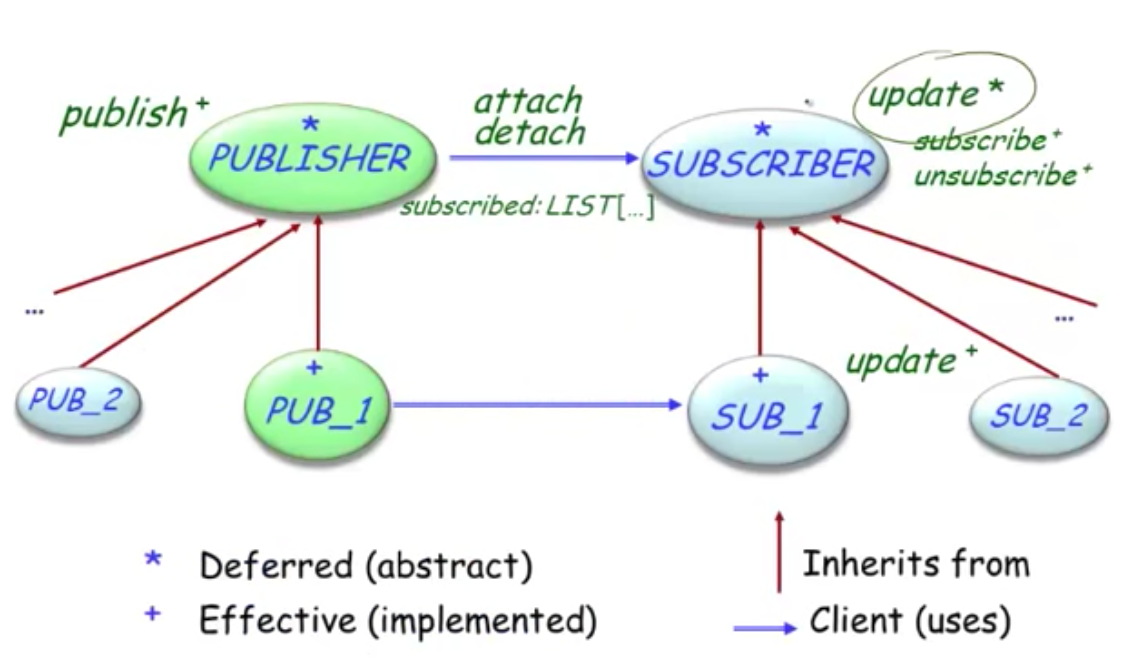
\includegraphics{pub}\\
The subscriber gets attached to the publisher an when the publisher publishes something new the subscriber is updated. Each publisher has a list of all the subscribers it has. A subscriber can subscribe itself to a publisher.\\Each subscriber has \hl{one} update operation and most of the time they are only subscribed to one publisher. Arguments(location of mouse etc...) can be passed to the update procedure.
\subsection{Beyond the observer pattern}
Since the publisher subscriber pattern is not reusable we will work on a new better one.
\subsubsection{The eiffel approach: the Event library}
In eiffel there is an event library. This class has only one type the \hl{event.} The \hl{context} is an object representing a user interface element, on which an event can take place. An event on a context makes an \hl{action} (a routine).\\While we program, we subscribe certain event type to certain action in a context.\\To declare an event:\\
click:EVENT\_TYPE[TUPLE[INTEGER,INTEGER]]\\create the event type:\\create click\\to trigger one occurence of the event:\\click.publish([x\_coordinate,y\_coordinate])\\on the subscriber side:\\click.subscribe (agent find\_station)\\A lot easier and reusable than the observer pattern. Another example:\\paris\_map.click.subscribe(agent find\_station)
\subsection{Tuples and agents}
\subsection{Tuples}
Tuples can be of many types for ex: Tuple[A,B,C] is a sequence of a least three values, first of type A, second B and third C. Like arrays but with multiple types. Is kind of like a class but with only fields(attributes). ex: TUPLE[author: STRING; year: INTEGER; title: STRING](the labels are optional). to access the fields t.year.
\subsection{Agents}
You can call the associated routine on an agent a through the feature call, whose argument is a single tuple: a.call([x\_pos, y\_pos]).\\
If a is associated with a function you call: a.item([..., ...]) this gives the result of applying the function.\\
for simplification you can omit these brackets []. You can also omit the .call and .item $\Rightarrow$ a(x,y,z), u := a(x,y,z) 
\subsubsection{Closed and open arguments}
u:= agent a0.f(a1,a2,a3)\\
z := agent a0.f(?,?,a3)\\
if all arguments are open you don't have to write the question marks.\\
u has all closed arguments(predefined) and we can call it with u.call   . Z has some open arguments, the ? which can defined while called z.cal(a1,a2)   .
\subsubsection{Declaring an agent}
p: PROCEDURE[C, TUPLE]\\
q: PROCEDURE[TUPLE[X,Y,Z], RES]\\
p has no open arguments, q has 3 open arguments and returns a result of type RES. C is type of target can be omitted $\Rightarrow$ TYPE ANY.







 




 


 




 















\end{document}
